% document formatting
\documentclass[10pt]{article}
\usepackage[utf8]{inputenc}
\usepackage[left=1in,right=1in,top=1in,bottom=1in]{geometry}
\usepackage[T1]{fontenc}
\usepackage{xcolor}

% math symbols, etc.
\usepackage{amsmath, amsfonts, amssymb, amsthm}

% lists
\usepackage{enumerate}

% images
\usepackage{graphicx} % for images

% code blocks
\usepackage{minted, listings} 

% verbatim greek
\usepackage{alphabeta}

\graphicspath{{./assets/images}}

\newcommand{\solution}{\textbf{Solution:}} 
\newcommand{\example}{\textbf{Example: }}

\title{EC ENGR 102 Week 3}

\author{Aidan Jan}
\date{\today}

\begin{document}
\maketitle

\subsection*{Memory}
\begin{itemize}
    \item A system has \textit{memory} if its output depends on past or future values of the input.  If the output depends only on present values of the input, the system is called \textit{memoryless}.
    \item e.g., $x(t) = A \cos(\omega t)$ is memoryless.
    \item $x(t) = \int_{-\infty}^t e^{-\tau^2} \text{d}\tau$ is not.
\end{itemize}

\subsection*{Invertibility}
\begin{itemize}
    \item A system is called \textit{invertible} if an input can always be exactly recovered from the output.  That is, a system $S$ is invertible if there exists an $S^{\text{inv}}$ such that
    \[x = S^{\text{inv}}(S(x))\]
    \item e.g., $y(t) = [x(t)]^2$ and $y(t) = \frac{\text{d}x(t)}{\text{d}t}$ are not invertible
    \item $y(t) = ax(t)$ for $a \neq 0$ is invertible.  Its inverse is $x(t) = \frac{1}{a} \cdot y(t)$.
\end{itemize}

\subsection*{System Impulse Response}
\begin{itemize}
    \item This lecture introduces time-domain analysis of systems, including the impulse response.  It also discusses linear time-invariant sysstems.  Topics include:
    \begin{itemize}
        \item Impulse response definition
        \item Impulse response of LTI systems
        \item The impulse response as a sufficient characterization of an LTI system
        \item Impulse response and the convolution integral
    \end{itemize}
    \item We've built a foundation on signal operations, signal models, and systems.  Today will be the first lecture where we present a new idea key to signals and systems: the impulse response.
    \item This impulse response will start us on the path to new concepts including convolution, Fourier series, and Fourier Transform
\end{itemize}

\section*{Impulse Response}
\subsection*{Why do we need the impulse response?}
\begin{itemize}
    \item In real life, we often do not have the luxury of knowing exactly what $S$ is, or perhaps we only know it imperfectly.  And even if we did know it, it could take on a very complicated form.
    \item The \textit{impulse response} is a characterization of the system that, for linear time-invariant systems, \textit{enables to calculate the output for \textbf{any} input}.  In this manner, it is a full time-domain description of the system.
\end{itemize}
\subsection*{Impulse Response Computation}
\[h(t) = H(\delta(t))\]
\begin{center}
    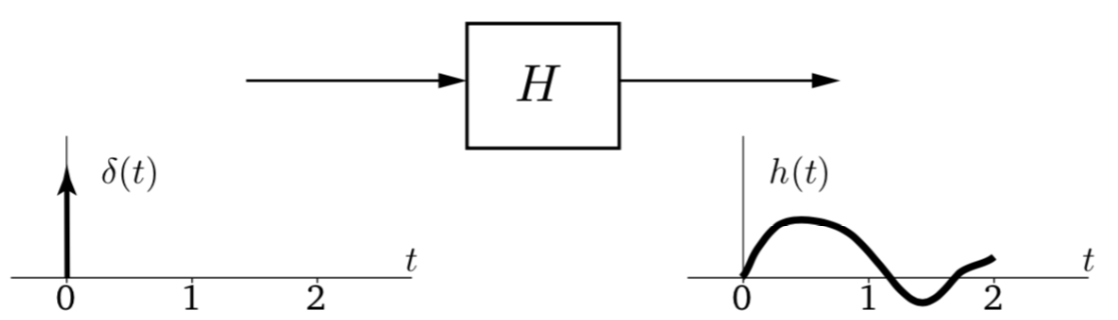
\includegraphics[scale=0.6]{W3_1.png}
\end{center}
\begin{itemize}
    \item In this case, our input signal is $x(t) = \delta(t)$, and our output is $y(t) = h(t)$.
\end{itemize}

\subsection*{Impulse response formal vs time invariant notation}
\underline{Formal:}
\begin{align*}
    y(t) &= H(x(t)) \\
    h(t) &= H(\delta(t)) \\
    h(t , \tau) &= H(\delta(t - \tau))
\end{align*}
\underline{Time-invariance:}
\begin{align*}
    h(t) &= H(\delta(t)) \\
    [FILL]
\end{align*}
\begin{center}
    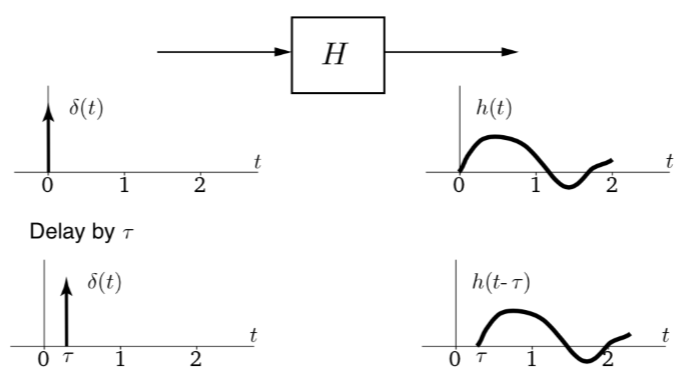
\includegraphics[scale=0.9]{W3_2.png}
\end{center}


\subsection*{A word on "t" in this formula}
\[h(t) = H(\delta(t))\]
In the above equation, the two $t$'s are NOT the same.
\begin{itemize}
    \item You cannot say $h(2) = H(\delta(2))$.
    \item The $t$ on the right is an independent variable that defines the input.
    \item The $t$ on the left is an independent variable that defines the output.
\end{itemize}
We can show this by making $h(t)$ the unit step function.  $h(2)$ would return 1, while $\delta(2)$ would return 0.

\subsection*{Extended Linearity}
Recall that a system, $H$, is linear if for $y_n = H(x_n)$ where $n$ is a subscript denoting different signals, and $a_n$ are constants, we have that:
\[\sum_n a_n y_n = H\left(\sum_n a_n x_n\right)\]
i.e., it has both homogeneity and superposition.  Thus, summation and the system operator can be interchanged.\\\\
In particular, this holds over integration (which is summation over infinitesimal intervals).  That is, if $y = H(x)$, then:
\[\int_{-\infty}^\infty a(\tau) y(t - \tau) \text{ d} \tau = H\left(\int_{-\infty}^\infty a(\tau) x(t - \tau) \text{ d}\tau\right)\]

\subsection*{Important fact about the impulse response}
\textbf{FACT:} If H is an LTI (linear time-invariant system) with impulse response
\[h(t) = H(\delta(t))\]
then we can calculate $H(x(t))$ for ANY $x(t)$ \textbf{\underline{IF}} we know $h(t)$.
\begin{itemize}
    \item Said differently, it is completely characterized by $h(t)$.  
    \item I can calculate $y(t)$ for \underline{any} $x(t)$ as long as I know $h(t)$.
\end{itemize}

\subsubsection*{Derivation of this fact}
Approach: write $x(t)$ in terms of $\delta(\tau)$'s.\\
Suppose $t = 0,\: x(0)$.
\[x(\tau) \cdot \delta(\tau) = x(0) \cdot \delta(\tau)\]
If we integrate this using the sampling property, we get $x(0)$.\\\\
If we now want to know what the value is at $x = 3$, then we do $t = 3,\:x(3)$.
\[x(\tau) \cdot \delta(\tau - 3) = x(3) \cdot \delta(\tau - 3)\]
By integrating this, we get the result of $x(3)$.\\\\
Now let's consider the general case: $x(t)$.
\[x(\tau) \cdot \delta(\tau - t) = x(t) \cdot \delta(\tau - t)\]
If we integrate this equation, we get $x(t)$.  Therefore, by sending an impulse through the circuit at particular values of $\tau$, we can find the result of the circuit.
\begin{align*}
    \int_{-\infty}^\infty x(\tau) \cdot \delta(\tau - t) \text{d}\tau &= \int_{-\infty}^\infty x(t) \cdot \delta(\tau - t) \text{d}\tau\\
    &= x(t) \cdot \int_{-\infty}^\infty \delta(\tau - t) \text{d}\tau\\
    &= x(t)
\end{align*}
We get the following two cases:
\begin{align*}
    x(t) &= \int_{-\infty}^\infty x(\tau) \delta(\tau - t) \text{d}\tau \\
    x(t) &= \int_{-\infty}^\infty x(\tau) \cdot \delta(t - \tau) \text{d}\tau
\end{align*}
From these two cases, we can assert that $\tau = t$.

\subsection*{The Convolution Integral}
\begin{align*}
    y(t) &= H(x(t))\\
    &= H\left(\int_{-\infty}^\infty x(\tau) \delta(t - \tau) \text{d}\tau\right)\\
    &= \int_{-\infty}^\infty x(\tau) H(\delta(t - \tau)) \text{d}t \hspace{2cm} \text{ this is possible since $H$ is linear}\\
    &= \int_{-\infty}^\infty x(\tau) \cdot h(t - \tau) \text{d}\tau \hspace{2cm} \text{H is time invariant.}
\end{align*}
If we now set the output to this function,
\[y(t) = \int_{-\infty}^\infty x(\tau) h(t - \tau) \text{d}\tau\]
This is called the "Convolution", or "Convolution integral".

\subsection*{Examples of computing the impulse response}
To find the impulse response,
\begin{enumerate}
    \item Set $x(t)$ to $\delta(t)$.
    \item We compute the system's output, $h(t) = H(\delta(t))$
\end{enumerate}
~\\
\underline{Example 1:}
What is the impulse response of $y(t) = \int_{-\infty}^t x(\tau) \text{d}\tau$?\\\\
\solution\\
It is the unit step function!
\begin{align*}
    h(t) &= \int_{-\infty}^t \delta(t) \text{d}\tau\\
    &= u(t)
\end{align*}
Note that $y(t) = \int_{-\infty}^\infty x(\tau) u(t - \tau) \text{d}\tau$, the convolution integral, is equal to the original $y(t)$ equation!\\\\
\underline{Example 2:}
\[y(t) = x(t - \alpha)\]
\solution\\
To find the impulse response, we apply the substitutions as described above:
\[h(t) = \delta(t - \alpha)\]

Looking at the convolution integral,
\begin{align*}
    y(t) &= \int_{-\infty}^\infty x(\tau) \cdot h(t - \tau) \text{d}\tau\\
    &= \int_{-\infty}^\infty x(\tau) \cdot \delta(t - T - \alpha) \text{d}\tau\\
    &= x(t - \alpha)
\end{align*}




\end{document}